% \documentclass[handout]{beamer} %"handout" serveix per a treure els \pause
\documentclass{beamer} %"handout" serveix per a treure els \pause
\usepackage{preamble}
\usepackage{../preamble_bib}

\addbibresource{references.bib} % add bibliography file.

\usetheme{Copenhagen}
\usecolortheme{seahorse}


%gets rid of bottom navigation bars
\setbeamertemplate{footline}[frame number]{}

%gets rid of bottom navigation symbols
\setbeamertemplate{navigation symbols}{}

% remove section and subsection from header
\setbeamertemplate{headline}{}

% set right and left margins
\setbeamersize{text margin left=10pt,text margin right=10pt}

\title{2D Turbulence spreading}
\author{
	Víctor Ballester\texorpdfstring{\vspace{0.45cm}\\}{}{\small Supervisors: Alexandros Alexakis (ENS)\texorpdfstring{\\}{}
\hspace{1.5cm} Emmanuel Dormy (ENS)}}
% \institute{Departament de Matemàtiques\\Facultat de Ciències}
\date{July XXXX, 2024}

% \def\myemph[#1]{
% \begingroup
% \textcolor{\mycolorhighlight}{#1}
% \endgroup}

\begin{document}
\thispagestyle{empty}
\frame[noframenumbering]{\titlepage}
% set the counter to 0
\setcounter{framenumber}{0}
\begin{frame}{Introduction}
	The aim of this work is to understand how turbulence spreads in a 2D incompressible fluid.

	This is motivated by the work of~\cite{alexakis}, where the author studied the spreading of turbulence in a long triply periodic domain. The natural questions that arise are:
	\begin{itemize}
		\item Do the vortices injected in the center of the domain spread til reaching the boundaries?
		\item If so, which profile does the energy and enstrophy distributions follow?
	\end{itemize}

	In this work, we tried to answer these questions in the 2D case.

	On top of that, we carried out a numerical simulation of the \textcolor{\mycolorhighlight}{point vortex model}, in order to compare and observe some similarities between the two models.
\end{frame}
\begin{frame}{Problem setup (Navier-Stokes)}
	We consider the \textcolor{\mycolorhighlight}{2D incompressible Navier-Stokes equations}, which after adimensionalizing read:
	\begin{align*}
		\partial_t \mathbf{u} + (\mathbf{u} \cdot \grad) \mathbf{u} & = -\grad p + \frac{1}{\text{Re}} \Delta \mathbf{u} + \mathbf{f} \\
		\divp \mathbf{u}                                            & = 0
	\end{align*}
	where $\mathbf{u}(\mathbf{x},t)$ is the velocity field, $p(\mathbf{x},t)$ is the pressure, $\Re$ is the Reynolds number, and $\mathbf{f}(\mathbf{x},t)$ is an external force.

	The force is localized in the center of the domain. Particularly, it injects vortices of sizes $\sim 1/k_\ell$ within a disk of size $\pi/k_r$. We do that in a way that the net momentum injected is zero.

	The Reynolds number is defined in terms of the length scale $1/k_\ell$ and the injection rate controlled by the amplitude of the force.
\end{frame}
\begin{frame}
	Thus, there are three parameters that control the dynamics of the system: $k_\ell$, $k_r$ and $\Re$. The following table summarizes the values used in the simulations:

	\begin{table}[ht]
		\centering
		\def\tickgreen{\textcolor{color_green3}{\ding{51}}}
		\def\tickblue{\textcolor{color_blue3}{\ding{51}}}
		% set space between columns
		\setlength{\tabcolsep}{3pt}
		% set space between rows
		\renewcommand{\arraystretch}{1.5}
		{\fontsize{8pt}{10pt}
			\begin{tabular}{c|cccccccccc}
				\diagbox[width=\dimexpr \textwidth/16+2\tabcolsep\relax, height=1cm]{$k_r$}{$\Re$} & 0.25               & 0.5                & 1                  & 2                           & 4                            & 8                            & 16                           & 32                           & 64                  & 128                 \\\hline
				8                                                                                  & \tickgreen$_{512}$ & \tickgreen$_{512}$ & \tickgreen$_{512}$ & \tickgreen\tickblue$_{512}$ & \tickgreen\tickblue$_{1024}$ & \tickgreen\tickblue$_{1024}$ & \tickgreen\tickblue$_{1024}$ & \tickgreen\tickblue$_{2048}$ & \tickgreen$_{2048}$ & \tickgreen$_{4096}$ \\
				16                                                                                 &                    &                    &                    & \tickblue$_{1024}$          & \tickblue$_{2048}$           & \tickgreen\tickblue$_{2048}$ & \tickgreen\tickblue$_{2048}$ & \tickgreen\tickblue$_{2048}$ & \tickgreen$_{4096}$ & \tickgreen$_{4096}$ \\
				32                                                                                 &                    &                    &                    & \tickblue$_{2048}$          & \tickblue$_{4096}$           & \tickgreen\tickblue$_{4096}$ & \tickgreen\tickblue$_{4096}$ & \tickgreen\tickblue$_{4096}$ & \tickgreen$_{8192}$ & \tickgreen$_{8192}$ \\
				64                                                                                 &                    &                    &                    &                             &                              & \tickgreen$_{8192}$          & \tickgreen$_{8192}$          & \tickgreen$_{8192}$          &                     &                     \\
			\end{tabular}}
		\caption{Simulations carried out during the study. \tickgreen = fully parallel simulations,\ \  \tickblue = embarrassingly parallel simulations.}\label{tab:simulations}
	\end{table}

	In all the simulations we set $k_\ell = 4 k_r$.
\end{frame}
\begin{frame}
	The quantities monitored during the simulations are the following:
	$$
		E_r      = \sum_{r-\Delta r<\norm{\vf{x}}\leq r} \norm{{\vf{u}}(\vf{x})}^2 \qquad
		\Omega_r = \sum_{r-\Delta r<\norm{\vf{x}}\leq r} \abs{{{\omega}}(\vf{x})}^2
	$$
	which account for the energy and enstrophy in annuli of radius $r$ and width $\Delta r$.

	We also defined a quantity that measures where most of the energy or enstrophy is located:
	$$
		\mathcal{R}_E^2      = \frac{\sum_{\Delta r<r\leq \pi} r^2 E_r}{\sum_{\Delta r<r\leq \pi} E_r}\qquad 	\mathcal{R}_\Omega^2 = \frac{\sum_{\Delta r<r\leq \pi} r^2 \Omega_r}{\sum_{\Delta r<r\leq \pi} \Omega_r}
	$$
\end{frame}
\begin{frame}{Problem setup (Point vortex)}
	We consider the most simple model of point vortices in 2D, which is based on the evolution by advection of a set of point where the vorticity $\omega$ is singular. In all the other points in $\RR^2$, the vorticity is zero.

	At all instants of time $\omega$ can be thought as a sum of Dirac deltas:
	\begin{equation*}
		\omega(\mathbf{x},t) = \sum_{i=1}^{N} \Gamma_i \delta(\mathbf{x} - \mathbf{x}_i(t))
	\end{equation*}
	where $\Gamma_i$ is the circulation of the $i$-th vortex, and $\mathbf{x}_i(t)$ is its position.

	A set of ODEs can be derived when imposed that they satisfy the 2D incompressible Euler equations:
	\begin{align*}
		\partial_t{\omega} + \vf{u} \cdot \grad {\omega} & = 0 \\
		\divp \vf{u}                                     & = 0
	\end{align*}
\end{frame}
\begin{frame}
	In the point vortex simulations, we input vortices in the center and remove them when they reach the boundaries.

	For this model, we monitor the number of vortices $N_r$ in annuli of radius $r$ and width $\Delta r$, in order to later on give an evolution of the linear density of number of vortices in rings of radius $r$:
	$$
		\rho_N(r) = \lim_{\Delta r\to 0} \frac{N_r}{2\pi r}
	$$

	We also monitor an equivalent \emph{mean radius} $\mathcal{R}_N$ weighted with the number of vortices in each annulus:
	$$
		\mathcal{R}_N^2 = \frac{\sum_{\Delta r<r\leq \pi} r N_r}{\sum_{\Delta r<r\leq \pi} N_r}
	$$
\end{frame}
\begin{frame}{Results}
	\begin{figure}[ht]
		\centering
		\begin{minipage}[t]{0.44\textwidth}
			\centering
			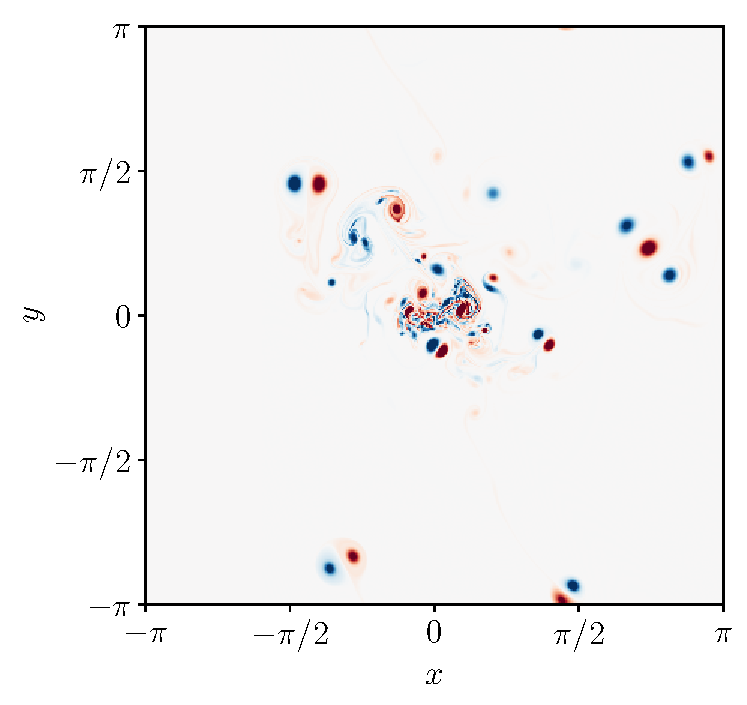
\includegraphics[width=\textwidth]{../images/domainRe128kdn16.pdf}
			\caption{Navier-Stokes simulation with $k_r = 16$ and $\Re = 128$.}
		\end{minipage}\hspace{0.04\textwidth}
		\begin{minipage}[t]{0.44\textwidth}
			\centering
			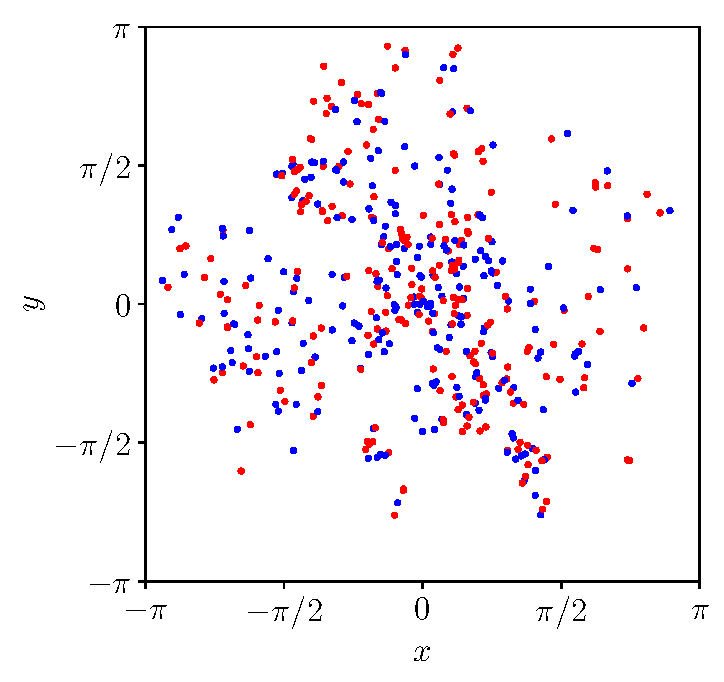
\includegraphics[width=\textwidth]{../images/pointvortices.R4.00440.pdf}
			\caption{Point vortex simulation with $k_r = 16$.}
		\end{minipage}
	\end{figure}
\end{frame}
\begin{frame}{Results (Navier-Stokes)}
	\begin{figure}[!ht]
		\centering
		\begin{subfigure}{0.44\textwidth}
			\centering
			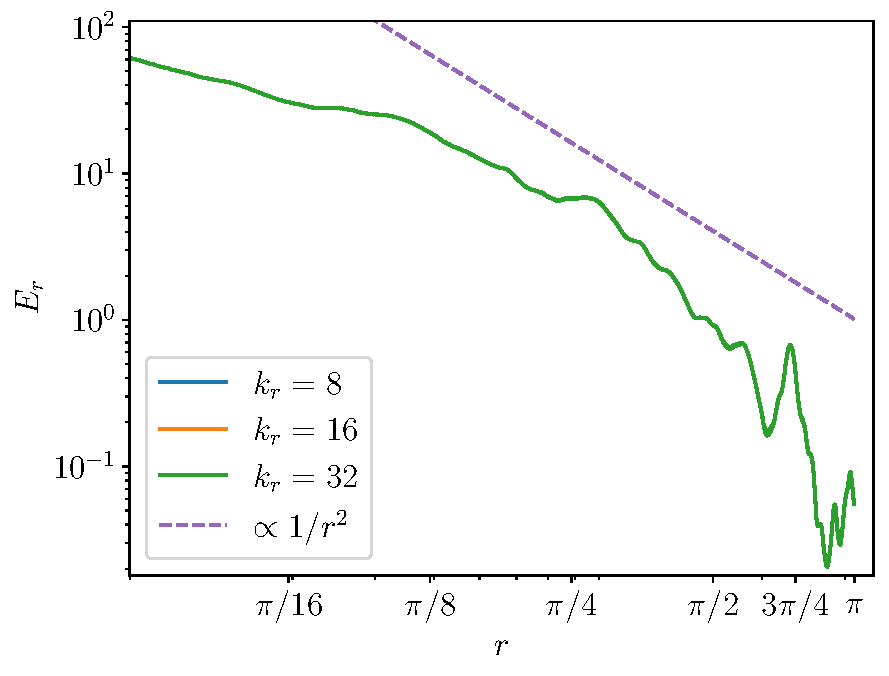
\includegraphics[width=\textwidth]{../images/Energy_kdn.test7.059.pdf}
			\caption{Energy profile}
		\end{subfigure}\hspace{0.04\textwidth}
		\begin{subfigure}{0.44\textwidth}
			\centering
			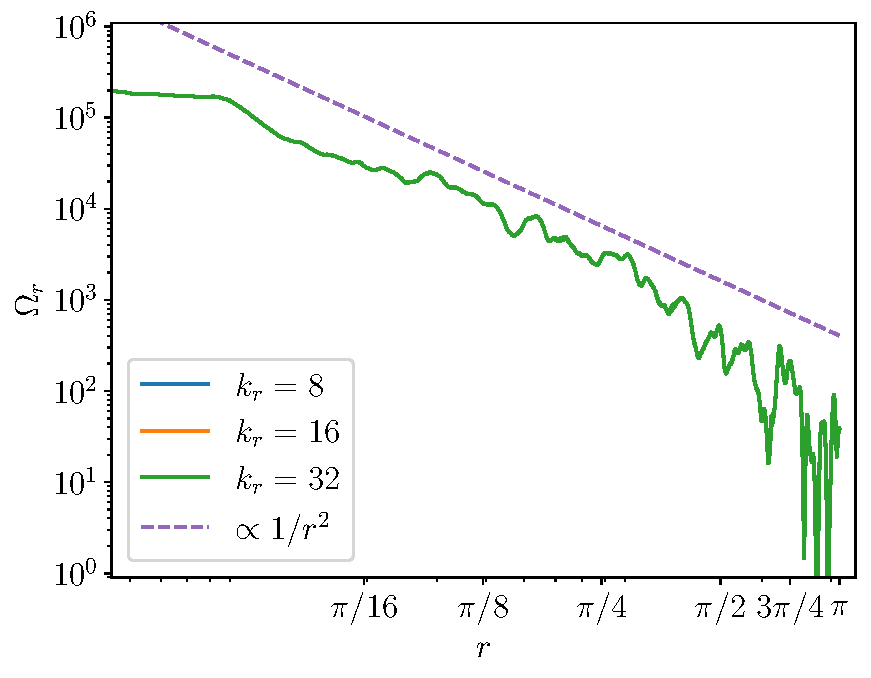
\includegraphics[width=\textwidth]{../images/Enstrophy_kdn.test7.059.pdf}
			\caption{Enstrophy profile}
		\end{subfigure}
		\caption{Energy and enstrophy profiles varying $k_r$ at fixed time and $\Re=32$.}
	\end{figure}
	\begin{itemize}
		\item Energy plots, smoother; enstrophy plots, more spiky.
		\item As $k_r$ increases, the apparent power law $A/r^2$ for the enstrophy extends.
	\end{itemize}
\end{frame}
\begin{frame}
	\begin{figure}[!ht]
		\begin{subfigure}{0.44\textwidth}
			\centering
			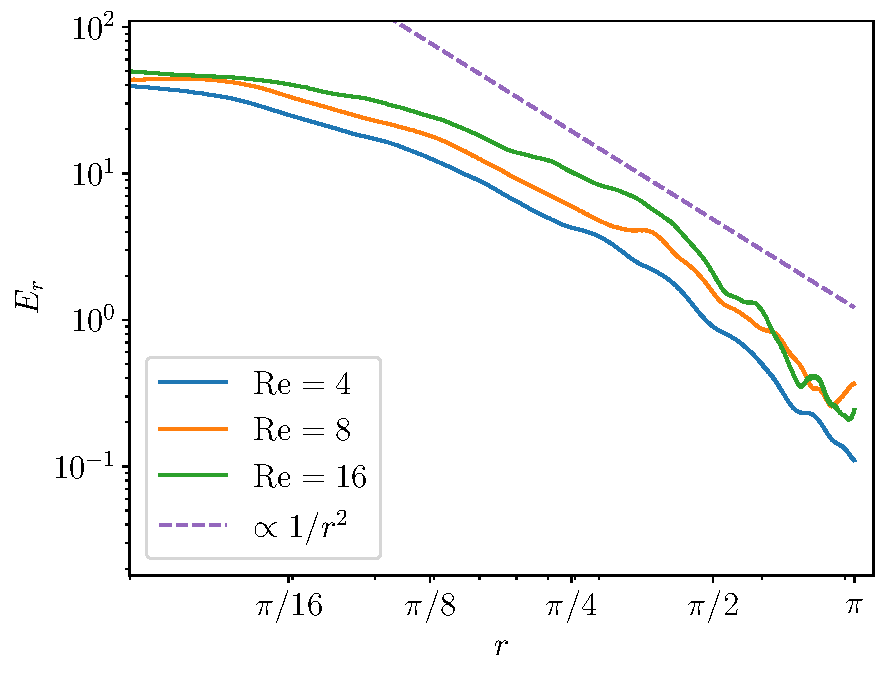
\includegraphics[width=\textwidth]{../images/Energy_Re.kdn16.175.pdf}
			\caption{Energy profile}
		\end{subfigure}\hspace{0.04\textwidth}
		\begin{subfigure}{0.44\textwidth}
			\centering
			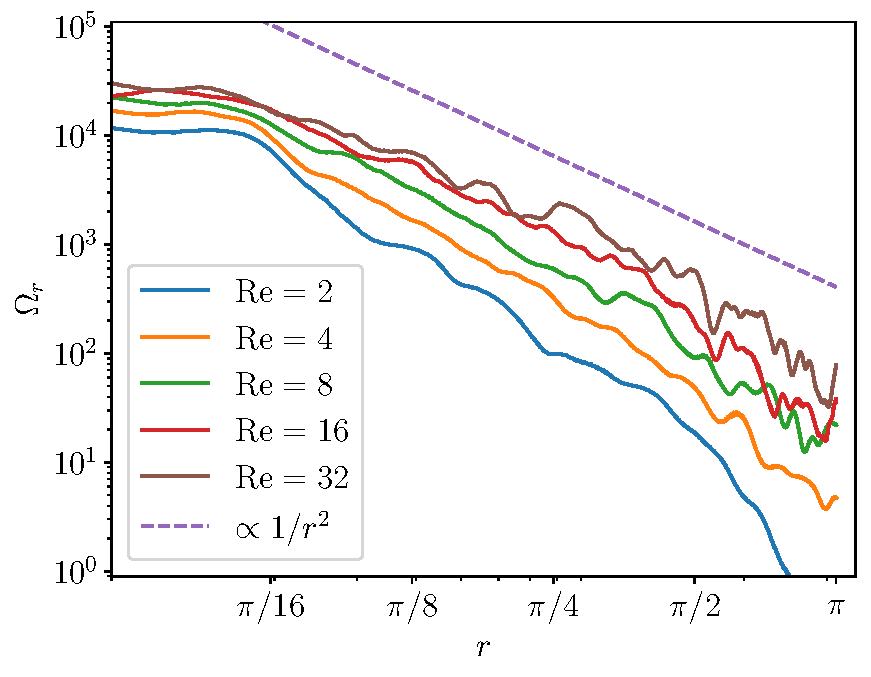
\includegraphics[width=\textwidth]{../images/Enstrophy_Re.kdn16.175.pdf}
			\caption{Enstrophy profile}
		\end{subfigure}
		\caption{Energy and enstrophy profiles varying $\Re$ at fixed time and $k_r=16$.}
	\end{figure}
	\begin{itemize}
		\item Again, energy plots are smoother than enstrophy plots.
		\item As $\Re$ increases, the magnitudes of both quantities increase due to less dissipation acting on the system.
	\end{itemize}
\end{frame}
\begin{frame}
	\begin{figure}[ht]
		\centering
		\begin{subfigure}{0.44\textwidth}
			\centering
			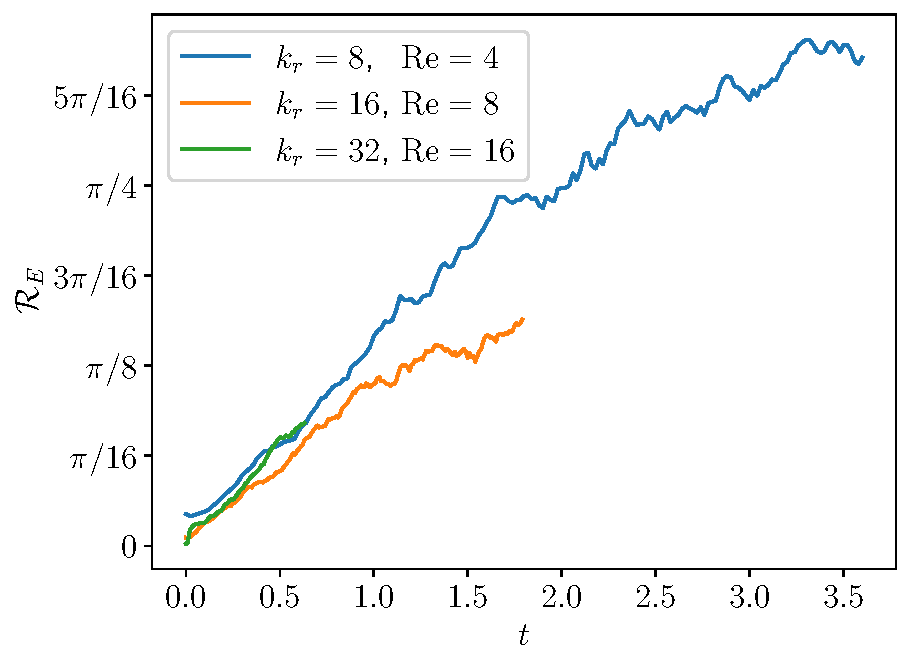
\includegraphics[width=\textwidth]{../images/EnergyMeanRadius.pdf}
			\caption{Energy mean radius}
		\end{subfigure}\hspace{0.04\textwidth}
		\begin{subfigure}{0.44\textwidth}
			\centering
			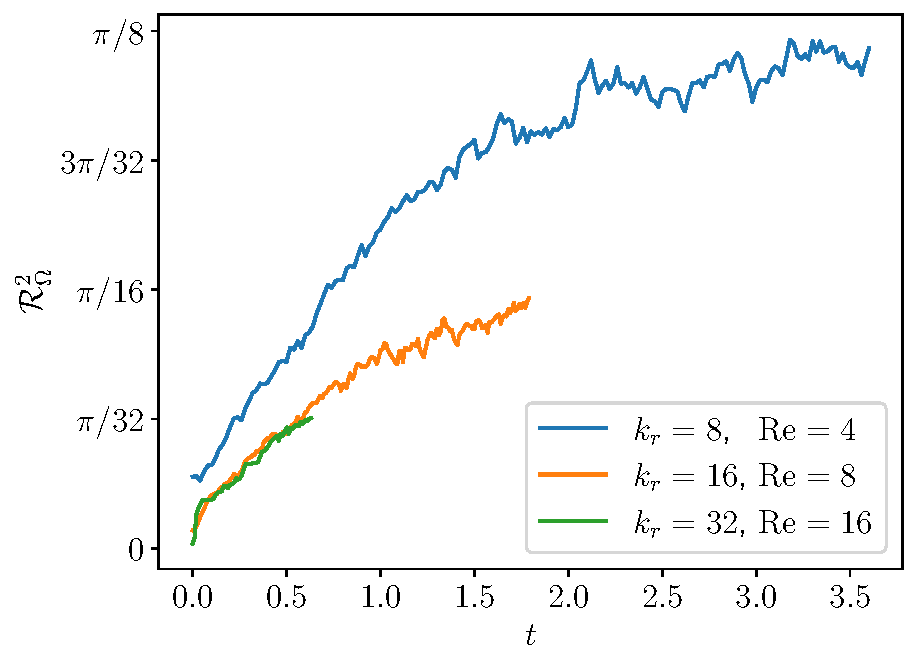
\includegraphics[width=\textwidth]{../images/EnstrophyMeanRadius.pdf}
			\caption{Enstrophy mean radius}
		\end{subfigure}
		\caption{Mean energy radius and mean enstrophy radius several runs varying simultaneously both $k_r$ and $\Re$.}
	\end{figure}
	\begin{itemize}
		\item $\mathcal{R}_E^2$ and $\mathcal{R}_\Omega^2$ increase with time, which means that vortices spread far from the perturbation region.
	\end{itemize}
\end{frame}
\begin{frame}{Results (Point vortex)}
	\begin{figure}[ht]
		\centering
		\begin{minipage}[t]{0.44\textwidth}
			\centering
			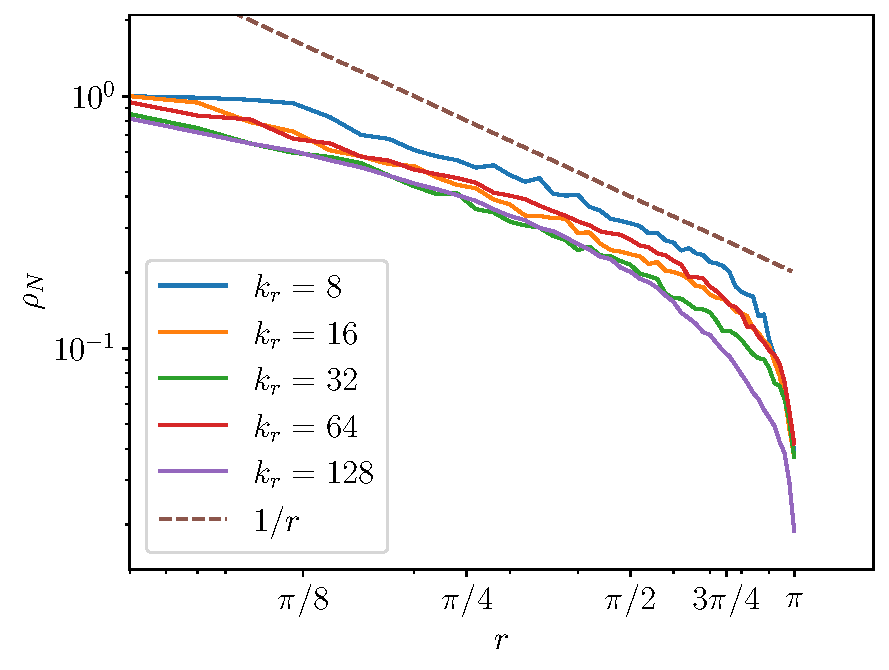
\includegraphics[width=\textwidth]{../images/NumVortices.pdf}
			\caption{Density of the number of vortices as a function of the radius.}
		\end{minipage}\hspace{0.04\textwidth}
		\begin{minipage}[t]{0.44\textwidth}
			\centering
			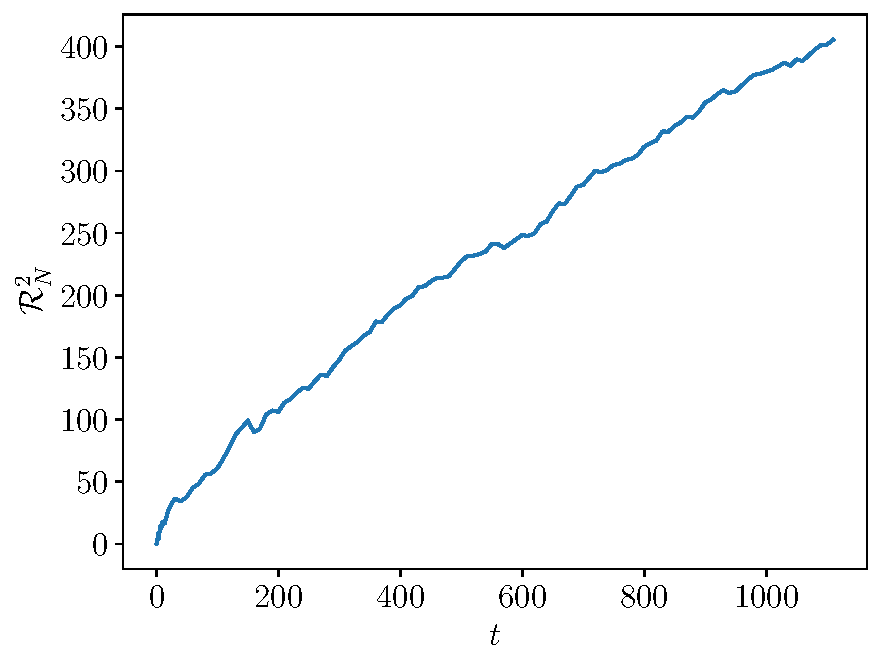
\includegraphics[width=\textwidth]{../images/NumVorticesMeanRadius.pdf}
			\caption{Mean radius weighted with the \#vortices as a function of time.}		\end{minipage}
	\end{figure}
	\vspace{-0.2cm}
	\begin{itemize}
		\item The density of vortices $\rho_N(r)$ following a power law $A/r$ in the middle range of $r$ implies that the flux of vortices on that region is almost constant.
		\item We observe an monotonous increase of $\mathcal{R}_N^2$ with time, which fits well with a linear function.
	\end{itemize}
\end{frame}
\begin{frame}{Conclusions}
	\begin{itemize}
		\item Energy injected in the center seems to spread across the domain, regardless of the size of the perturbation region if the Reynolds number is high enough.
		\item The enstrophy seems to follow a power law $A/r^2$, that for large $k_r$ and enough time, extends to the whole domain.
		\item When a stationary state is reached for the point vortex model, we observe a constant flux of vortices in the middle range of $r$.
	\end{itemize}

	Improvements to be done:
	\begin{itemize}
		\item Integrate the Navier-Stokes simulation further in time.
		\item Simulate the cases for $k_r= 64$ and higher Reynolds numbers.
		\item Replicate the results adding a drag term $-\alpha \vf{u}$ to the equations. Can we conclude the same?
	\end{itemize}
\end{frame}

\thispagestyle{empty}
\begin{frame}[noframenumbering]{Bibliography}
	\printbibliography
	\vspace{4cm}
\end{frame}
\end{document}
